\documentclass[11pt]{article} \usepackage[top=1in, bottom=1in, left=1in, right=1in]{geometry}
\usepackage{amsfonts, amsmath, amssymb, amsthm}
\usepackage{xcolor}
\usepackage{hyperref}
\usepackage[british,calc]{datetime2}
\usepackage{advdate}
\usepackage{tikz}
\usepackage{booktabs}
\usepackage{float}
\bibliographystyle{ieeetr}

\title{Surgical Phase Detection Using Deep Learning\\ Critical Review}
\author{Xiaorui Zhang, Wenkai Luo, Xucheng Ma}
\date{March 2022}

\begin{document}
\maketitle
\section{Project Problem Statement \& Background}
Our project focuses on developing Deep Learning models which perform mastoidectomy video segmentation. The model \textbf{inputs} is a sequence of frames, and model \textbf{output} is a sequence of surgical phase labels. The main technical problems we need to solve is how to design an efficient and robust feature extractor for surgical videos, then we can perform classification in the feature space to obtain phase labels.

\vspace{0.25cm}
\noindent
In general surgical phase segmentation workflow, both \textbf{spatial} features and \textbf{temporal} features are often considered, e.g.
\begin{itemize}
  \item Spatial Features: anatomical structures, tool presence/positioning ...
  \item Temporal Features: anatomical changes, tool movement, camera view changes​ ...
\end{itemize}
Mastoidectomy videos has some characteristic features:
\begin{itemize}
  \item Anatomical features are mostly \textbf{rigid} since is a skull based surgery.
  \item Anatomical changes are mostly in depth direction as the overall surgery process is exposing the interior structures behind patient's ear.
  \item Camera view changes might imply transition between surgical phases.
  \item Tool positioning may contain more useful information about correct phase label than tool presence, because main tools involved are only drill and suction device and the are used across whole procedure.
\end{itemize}

\vspace{0.25cm}
\noindent
Typical DL methods for surgical phase segmentation has following components:
\begin{itemize}
  \item Spatial Feature Extractor
  \item Temporal Feature Extractor
  \item Spatial-Temporal Feature Fusion
  \item Classifier in Feature Space
\end{itemize}
Papers which we included in this review are all consisted of components above, but different approaches were chosen for each component. For each paper, we first introduce the problem that the specific network design aimed to address, then summarize the main contributions, and discuss key results and potential problems.

\section{Critical Review of SV-RCNet}
\subsection{Background and problems with prior works}
The automatic surgical video segmentation is a fundamental component in building a context-awareness computer-aided surgery system.  Before this work, several Vision-Based and Deep Learning oriented methods were proposed to extract spatial and temporal features and train a classifier to perform the segmentation task. However, there are three main drawbacks to the previous works.  First, the previously used visual features, either hand-crafted or shallow CNN-based, are still far from sufficient to represent the complicated visual characteristics of the frames in surgical videos. In addition, when exploiting the temporal information, most traditional methods rely on linear statistical models with pre-defined dependencies, which are incapable of precisely representing motions in the surgical videos, especially for frame series with strong non-linear dynamics. Second, and more importantly, most existing methods harness visual and temporal information separately, i.e., first using visual features with classifiers to predict each frame, and then using temporal dependencies to refine the results. In this way, visual features are unable to play a role in the temporal model and therefore such a scheme hardly benefits from the Spatio-Temporal information. Third, due to the above-mentioned two reasons, we analyze and find that it would be difficult for previous methods to sensitively identify and locate the transition frames while recognizing which is very important to achieve accurate and consistent workflow recognition results. \cite{SV-RCNet}
\subsection{Significance of this paper}
There are three main contributions from this paper. First, this paper proposed for the first time to use a deep neural network to extract visual features from the video frames. The ResNet makes it possible to optimize a much deeper network by embedding the identity transformation into the network through residual blocks. Using the ResNet as a spatial feature extractor, the SV-RCNet is able to find more discriminative features compared with models of shallow CNN. Second, instead of dealing with spatial and temporal features separately, SV-RCNet integrates ResNet and LSTM to form a novel recurrent convolutional architecture in order to take full advantage of the complementary information of visual and temporal features. LSTM is a direct improvement on the top of recurrent neural network (RNN), LSTM uses gates to generate “cell states” to aid the gradient flow and alleviate vanishing gradient. LSTM is designed to avoid long-term dependency problems and makes the training of long sequential data possible. SV-RCNet integrates the ResNet and the LSTM network, so that they are jointly trained in an end-to-end manner to generate high-level features that encode both spatial (visual) and temporal information. Particularly, the Spatio-temporal features learned by SV-RCNet are sensitive to motions in surgical videos and can precisely identify the phase transition frames. Third, considering that the results produced from SV-RCNet are transition-sensitive and the surgical videos are well-structured, another simple yet effective scheme called prior knowledge inference (PKI) is proposed to refine the SV-RCNet output. The PKI strategy is tailored to make use of the natural characteristics of surgical videos and can greatly improve recognition accuracy.
\subsection{Results and problems}
SV-RCNet was the state-of-the-art model in surgical video segmentation in terms of performance in both Cholec80 and MICCAI M2CAI workflow Challenge. However, there are still drawbacks inherited in LSTMs, which retain the memory of a limited sequence, that cannot span minutes or hours, which is the average duration of surgery. Thus, the temporal information must be present in a slow, sequential way and prohibits inference parallelization, which would be beneficial for integration in an online OR scenario.


\section{Critical Review of Trans-SVNet}
\subsection{Problem with previous work and proposed method}
As shown in figure \ref{fig:transsvnet_structure} (a), previous methods perform spatial and temporal feature extractions in serial, where CNN-based methods serves as spatial feature extractor, and the resulting features are then fed into temporal feature extractor; there's no specific module in the network that fuse the spatial and temporal features. The spatial-temporal representations obtained by successive spatial and temporal feature extractions overlook the complementary effects of spatial and temporal features. \cite{TransSVNet}.

\begin{figure}[H]
  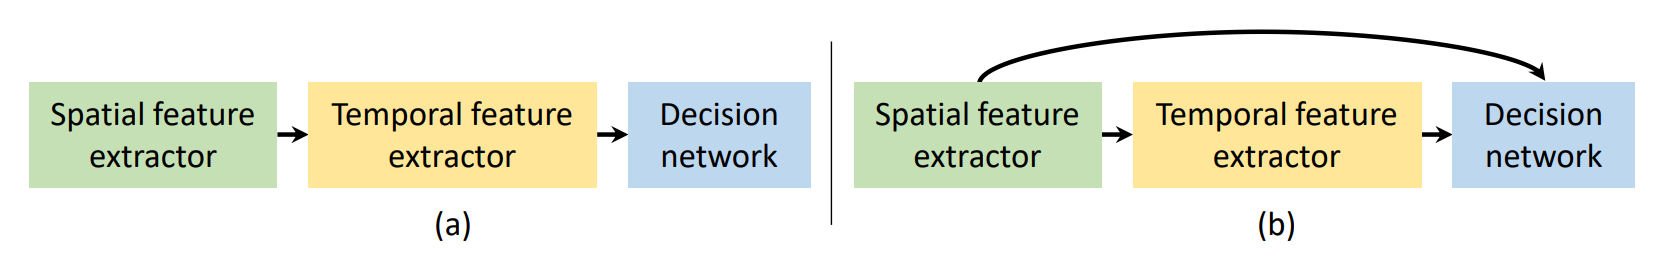
\includegraphics[width=\textwidth]{trans_svnet_1.png}
  \centering
  \caption{ Structure of methods for surgical phase segmentation: (a) previous works (b) Trans-SVNet \cite{TransSVNet}}
  \label{fig:transsvnet_structure}
\end{figure}

\vspace{0.25cm}
\noindent
In Trans-SVNet, transformer layer is used as an aggregation model which fuses spatial and temporal features, and it serves as the decision network mentioned in figure \ref{fig:transsvnet_structure}. Figure \ref{fig:transsvnet_network} shows the network architecture.

\begin{figure}[H]
  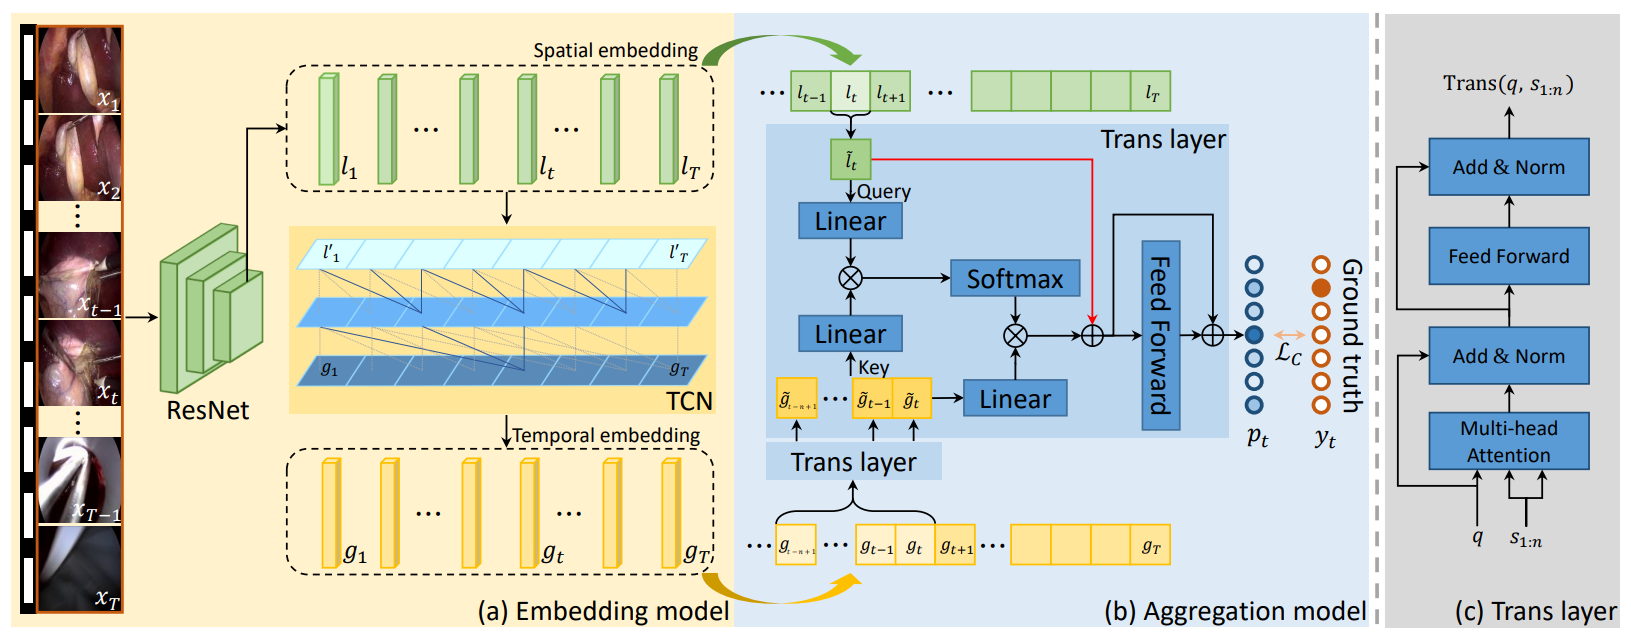
\includegraphics[width=\textwidth]{trans_svnet_2.png}
  \centering
  \caption{ Trans-SVNet architecture\cite{TransSVNet}}
  \label{fig:transsvnet_network}
\end{figure}

\vspace{0.25cm}
\noindent
The network use ResNet as the spatial feature extractor; temporal features are then extracted with TeCNO from spatial features. The first transformer layer of the aggregation model (not shown in figure \ref{fig:transsvnet_network}) performs self-attention on sequence of temporal features , then the second transformer layer performs a cross-attention where dimensionally reduced spatial features are queries, and the resulting temporal features from previous transformer layer are both keys and values. The output features is a weighted sum of temporal features in the sequence, where the weights contains information of the relations between corresponding spatial feature and other temporal features in the sequence.

\subsection{Contributions and experiment results}
The main contributions of this paper are summarized as followings:
\begin{itemize}
  \item It's the first time that transformer is used to reconsider the Complementary Effects of spatial and temporal features.
  \item A significant boost in inference speed is achieved by processing hybrid embeddings in parallel
\end{itemize}
The experiment results on Cholec80 and M2CAI16 are shown in table \ref{fig:transsvnet_result}, and we can see that Trans-SVNet outperforms other state-of-arts methods while keeping a relative low number of parameters.
\begin{figure}[H]
  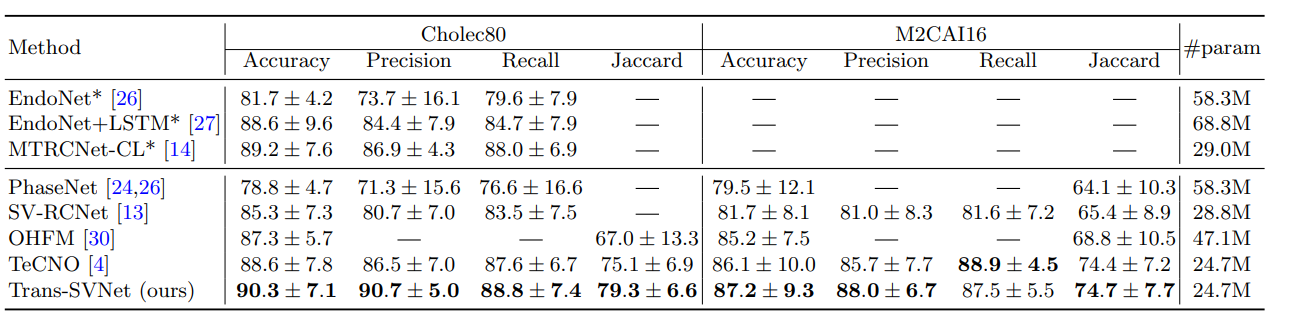
\includegraphics[width=\textwidth]{trans_svnet_3.png}
  \centering
  \caption{Experiment Results on Cholec80 and M2CAI16}
  \label{fig:transsvnet_result}
\end{figure}

\subsection{Assessment and future work}
As for our project, this paper inspires us that attention mechanism provides a good way to fuse spatial and temporal features; moreover, the attention mechanism can also be use to fuse any sequence of features. Another valuable knowledge we learn from this paper is that low-dimensional video embeddings result in significant inference speed boost, but we should be aware that this is under the assumption that image frames with same surgical labels do cluster in the spatial feature space.

\vspace{0.25cm}
\noindent
On the other hands, there are some debatable points in this paper. The embedding model (2 feature extractors) and aggregation model (transformer layer) are trained separately, and there is no comparison between the proposed method and results from running transformer-based method directly on spatial features. To address these two concerns and build our network based on Trans-SVNet, we are planning to first compare Trans-SVNet with end-to-end trained models and pure-spatial features model, and then treat "idle" and "camera adjustment" as different tasks instead of labels and use cross-attention to exploring the complementary effects of "idle"/"camera adjustment" and the main surgical phase segmentation task.

\newpage
\bibliography{bibfile}
\end{document}